
\documentclass[12pt,a4paper]{article}% 文档格式
\usepackage{ctex,hyperref}% 输出汉字
\usepackage{times}% 英文使用Times New Roman
%%%%%%%%%%%%%%%%%%%%%%%%%%%%%%%%%%%%%%%%%%%%%%%%%%%%%%%%
\title{\fontsize{18pt}{27pt}\selectfont% 小四字号,1.5倍行距
    {\heiti% 黑体
        计算物理——Homework Week 11}}% 题目
%%%%%%%%%%%%%%%%%%%%%%%%%%%%%%%%%%%%%%%%%%%%%%%%%%%%%%%%
\author{\fontsize{12pt}{18pt}\selectfont% 小四字号,1.5倍行距
    {\fangsong% 仿宋
        白博臣、何骐多、夏营}\\% 标题栏脚注
    \fontsize{10.5pt}{15.75pt}\selectfont% 五号字号,1.5倍行距
    {\fangsong% 仿宋
        (四川大学~~~物理学拔尖计划)}}% 作者单位,“~”表示空格
%%%%%%%%%%%%%%%%%%%%%%%%%%%%%%%%%%%%%%%%%%%%%%%%%%%%%%%%
\date{}% 日期(这里避免生成日期)
%%%%%%%%%%%%%%%%%%%%%%%%%%%%%%%%%%%%%%%%%%%%%%%%%%%%%%%%
\usepackage{amsmath,amsfonts,amssymb}% 为公式输入创造条件的宏包
%%%%%%%%%%%%%%%%%%%%%%%%%%%%%%%%%%%%%%%%%%%%%%%%%%%%%%%%
\usepackage{graphicx}% 图片插入宏包
\usepackage{subfigure}% 并排子图
\usepackage{float}% 浮动环境,用于调整图片位置
\usepackage[export]{adjustbox}% 防止过宽的图片
%%%%%%%%%%%%%%%%%%%%%%%%%%%%%%%%%%%%%%%%%%%%%%%%%%%%%%%%
\usepackage{bibentry}
\usepackage{natbib}% 以上2个为参考文献宏包
%%%%%%%%%%%%%%%%%%%%%%%%%%%%%%%%%%%%%%%%%%%%%%%%%%%%%%%%
\usepackage{abstract}% 两栏文档,一栏摘要及关键字宏包
\renewcommand{\abstracttextfont}{\fangsong}% 摘要内容字体为仿宋
\renewcommand{\abstractname}{\textbf{摘\quad 要}}% 更改摘要二字的样式
%%%%%%%%%%%%%%%%%%%%%%%%%%%%%%%%%%%%%%%%%%%%%%%%%%%%%%%%
\usepackage{xcolor}% 字体颜色宏包
\newcommand{\red}[1]{\textcolor[rgb]{1.00,0.00,0.00}{#1}}
\newcommand{\blue}[1]{\textcolor[rgb]{0.00,0.00,1.00}{#1}}
\newcommand{\green}[1]{\textcolor[rgb]{0.00,1.00,0.00}{#1}}
\newcommand{\darkblue}[1]
{\textcolor[rgb]{0.00,0.00,0.50}{#1}}
\newcommand{\darkgreen}[1]
{\textcolor[rgb]{0.00,0.37,0.00}{#1}}
\newcommand{\darkred}[1]{\textcolor[rgb]{0.60,0.00,0.00}{#1}}
\newcommand{\brown}[1]{\textcolor[rgb]{0.50,0.30,0.00}{#1}}
\newcommand{\purple}[1]{\textcolor[rgb]{0.50,0.00,0.50}{#1}}% 为使用方便而编辑的新指令
%%%%%%%%%%%%%%%%%%%%%%%%%%%%%%%%%%%%%%%%%%%%%%%%%%%%%%%%
\usepackage{url}% 超链接
\usepackage{bm}% 加粗部分公式
\usepackage{multirow}
\usepackage{booktabs}
\usepackage{svg}
\usepackage{epstopdf}
\usepackage{epsfig}
\usepackage{longtable}% 长表格
\usepackage{supertabular}% 跨页表格
\usepackage{algorithm}
\usepackage{algorithmic}
\usepackage{changepage}% 换页
%%%%%%%%%%%%%%%%%%%%%%%%%%%%%%%%%%%%%%%%%%%%%%%%%%%%%%%%
\usepackage{enumerate}% 短编号
\usepackage{caption}% 设置标题
\captionsetup[figure]{name=\fontsize{10pt}{15pt}\selectfont Figure}% 设置图片编号头
\captionsetup[table]{name=\fontsize{10pt}{15pt}\selectfont Table}% 设置表格编号头
%%%%%%%%%%%%%%%%%%%%%%%%%%%%%%%%%%%%%%%%%%%%%%%%%%%%%%%%
\usepackage{indentfirst}% 中文首行缩进
\usepackage[left=2.50cm,right=2.50cm,top=2.80cm,bottom=2.50cm]{geometry}% 页边距设置
\renewcommand{\baselinestretch}{1.5}% 定义行间距(1.5)
%%%%%%%%%%%%%%%%%%%%%%%%%%%%%%%%%%%%%%%%%%%%%%%%%%%%%%%%
\usepackage{fancyhdr} %设置全文页眉、页脚的格式
\pagestyle{fancy}
\hypersetup{colorlinks=true,linkcolor=black}% 去除引用红框,改变颜色

% Packages
\usepackage{geometry}
\usepackage{listings}
\usepackage{xcolor}
\usepackage{graphicx}
\usepackage{amsmath}
\usepackage{subcaption}
\usepackage{mathtools}

%%%%%%%%%%%%%%%%%%%%%%%%%%%%%%%%%%%%%%%%%%%%%%%%%%%%%%%%
\newtheorem{theorem}{\indent 定理}[section]
\newtheorem{lemma}[theorem]{\indent 引理}
\newtheorem{proposition}[theorem]{\indent 命题}
\newtheorem{corollary}[theorem]{\indent 推论}
\newtheorem{definition}{\indent 定义}[section]
\newtheorem{example}{\indent 例}[section]
\newtheorem{remark}{\indent 注}[section]
\newenvironment{solution}{\begin{proof}[\indent\bf 解]}{\end{proof}}
\renewcommand{\proofname}{\indent\bf 证明}

%%%%%%%%%%%%%%%%%%%%%%%%%%%%%%%%%%%%%%%%%%%%%%%%%%%%%%%%

\begin{document}% 以下为正文内容
\maketitle% 产生标题,没有它无法显示标题
%%%%%%%%%%%%%%%%%%%%%%%%%%%%%%%%%%%%%%%%%%%%%%%%%%%%%%%%
\lhead{}% 页眉左边设为空
\chead{}% 页眉中间设为空
\rhead{}% 页眉右边设为空
\lfoot{}% 页脚左边设为空
\cfoot{\thepage}% 页脚中间显示页码
\rfoot{}% 页脚右边设为空
%%%%%%%%%%%%%%%%%%%%%%%%%%%%%%%%%%%%%%%%%%%%%%%%%%%%%%%%
\begin{figure}[h]
    \centering
    \begin{minipage}{0.32\textwidth}
        \centering
        \includegraphics[width=\linewidth]{bbc}
        \caption{白博臣}
        \label{白博臣照片}
    \end{minipage}\hfill
    \begin{minipage}{0.305\textwidth}
        \centering
        \includegraphics[width=\linewidth]{hqd}
        \caption{何骐多}
        \label{何骐多照片}
    \end{minipage}\hfill
    \begin{minipage}{0.32\textwidth}
        \centering
        \includegraphics[width=\linewidth]{xy}
        \caption{夏营}
        \label{夏营照片}
    \end{minipage}
\end{figure}


%    \begin{center}% 居中处理
%    {\textbf{Abstract}}% 英文摘要
%    \end{center}
%    \begin{adjustwidth}{1.06cm}{1.06cm}% 英文摘要内容
%        \hspace{1.5em}Attention!If you input "dif{}ferent", the computer will output "different", but if you input "dif\{\}ferent", the computer will output "dif{}ferent"
%    \end{adjustwidth}
\newpage% 从新的一页继续

\section{Probelm 1}
\subsection{题目回顾}
用传统的MC方法模拟蒲丰投针问题,并进行计算$\pi$值。

$\left(a\right)$ 在固定N下改变x$\left(x=b/a\right) x=b/a $的值,讨论影响最终结果的因素,解释$\pi$的估计值的精度往往随着针头长度的增加而提高。(为了简单起见,选择a=1)

$\left(b\right)$ 固定x的取值,增加投针次数N,观察$\pi$的估计值的变化情况。

$\left(c\right)$ 讨论一下为什么电脑只能达到这个精度?

$\left(d\right)$ 如果我们定义$x=a/b$,这就是长度增加的针头的概率函数,选择$x=1,2,3\dots14$等,能否正确估计$\pi$值,将结果打印出来并生成计算$\pi$值最佳的x值。

\begin{figure}[htbp]
    \centering
    \includegraphics[height=0.4 \textheight]{蒲丰投针示意图.pdf}
    \caption{蒲丰投针实验示意图}\label{投针示意图}
\end{figure}

\subsection{问题解答}
\subsubsection{问题$\left(a\right)$解答}

蒲丰实验生成n个服从$U(0,\pi)$的随机数$\theta$和n个服从$U(0,\frac{a}{2})$的随机数,令$k$为实验成功的次数,初始为0,对于每对随机数$(\theta,x)$,如果$x\leq \frac{l*sin \theta}{2}$,那么实验就视为成功,$k$加1.因此最后针与木条相交的概率$P=\frac{k}{n}$,从而可得$\pi$的估计值$\hat{\pi}=\frac{2ln}{ak}$.样本点在广义空间的分布情况如下图所示:

\begin{figure}[htbp]
    \centering
    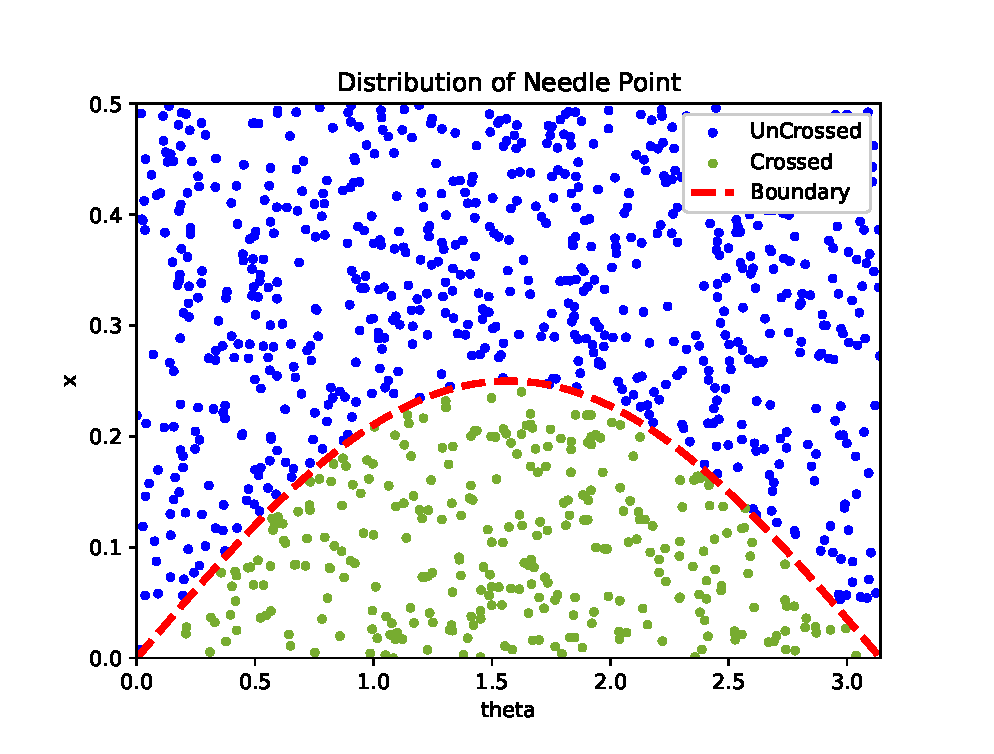
\includegraphics[height=8cm]{样本点示意图.eps}\label{样本点分布图}
    \caption{1000个样本点的分布示意图}
\end{figure}

使用Python编程得到$\pi(x)$随$x$的变化情况,并绘制出相对误差分布如下图所示:

\begin{figure}[H]% 插入两张图片并且并排
    \centering
    \begin{minipage}{0.48\textwidth}
        \centering
        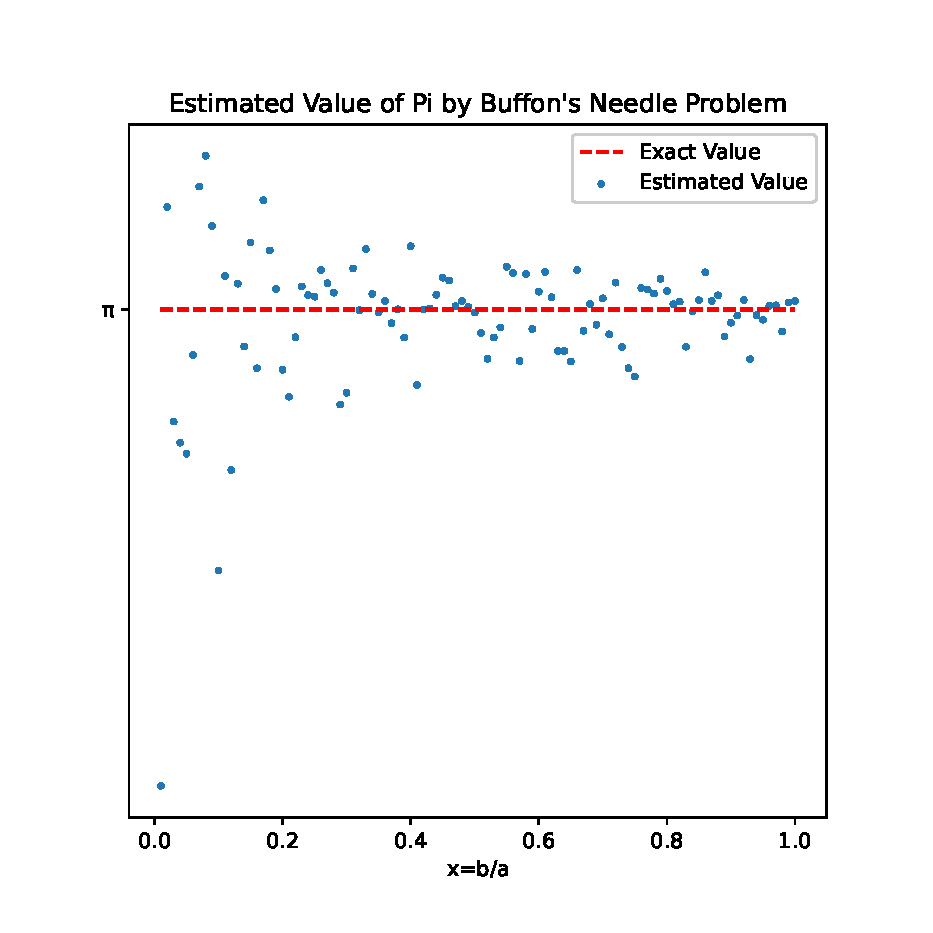
\includegraphics[width=1.1\textwidth]{Pi_value.eps}
        \caption{\fontsize{10pt}{15pt}\selectfont $\pi(x)$随$x$变化示意图}
    \end{minipage}
    \hspace{0cm}% 图片间距
    \hfill% 撑满整行
    \begin{minipage}{0.48\textwidth}
        \centering
        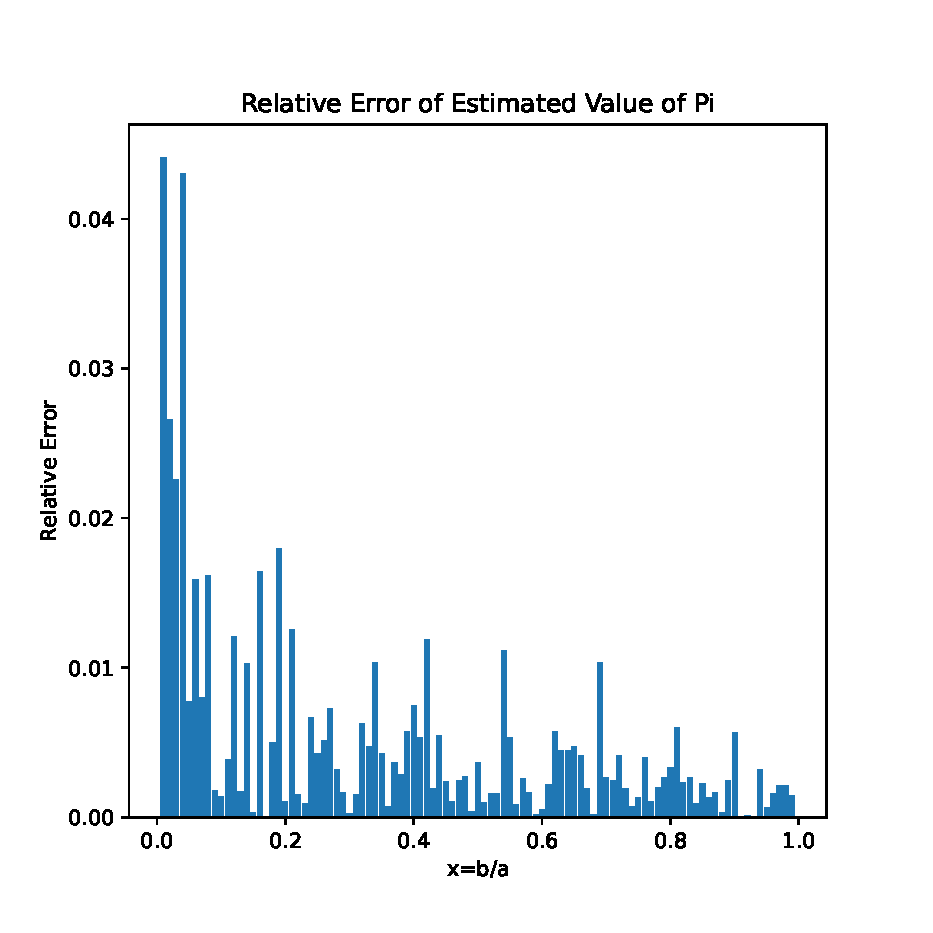
\includegraphics[width=1.1\textwidth]{Relative Error.eps}
        \caption{\fontsize{10pt}{15pt}\selectfont 相对误差分布图}
    \end{minipage}\label{fig:figure2}
\end{figure}

我们观察到,随着$x$值的增加,$\pi$的估计值的精度有逐渐提高的趋势,说明在投针次数$N$固定的条件下,针的长度应该和地板的长度相匹配,才能在单词实验中获得最优的估计结果。

从经验的角度分析,一方面Monte Carlo方法要以高精度实现对参数的估计,需要尽可能满足样本分布的随机性,即针的分布应该足够均匀,针覆盖区域的面积应该足够大,由于针并非质点,故针的长度会影响覆盖区域面积的均匀性。当针越长的时候,其均匀性也就越好,最终的估计值也就越精确。

另一方面,本实验主要有三个参数:针与地板的夹角$\theta$以及针的质心位置$(x,y)$,如果想要达到分布的均匀,就要要求三个参数固定两个参数时,另一个参数的变化要引起结果的变化,否则便会出现样本的重复累计,破坏样本的均匀性。当我们固定质心坐标$(x,y)$,当针比较长的时候,改变$\theta$的取值便会出现针与线相交情况的改变;当针比较短的时候,改变$\theta$并不会改变针与线的相交情况,这就导致了参数的随机性并没有带来结果的随机性。所以当针的长度增加时,$\pi$的估计值的精度也在提高。

\subsubsection{问题$\left(b\right)$解答}
使用Python编写投针程序,得到估计结果$\pi(N)$随着投掷次数$N$的变化情况及其相对误差分布如下图所示:

\begin{figure}[H]% 插入两张图片并且并排
    \centering
    \begin{minipage}{0.48\textwidth}
        \centering
        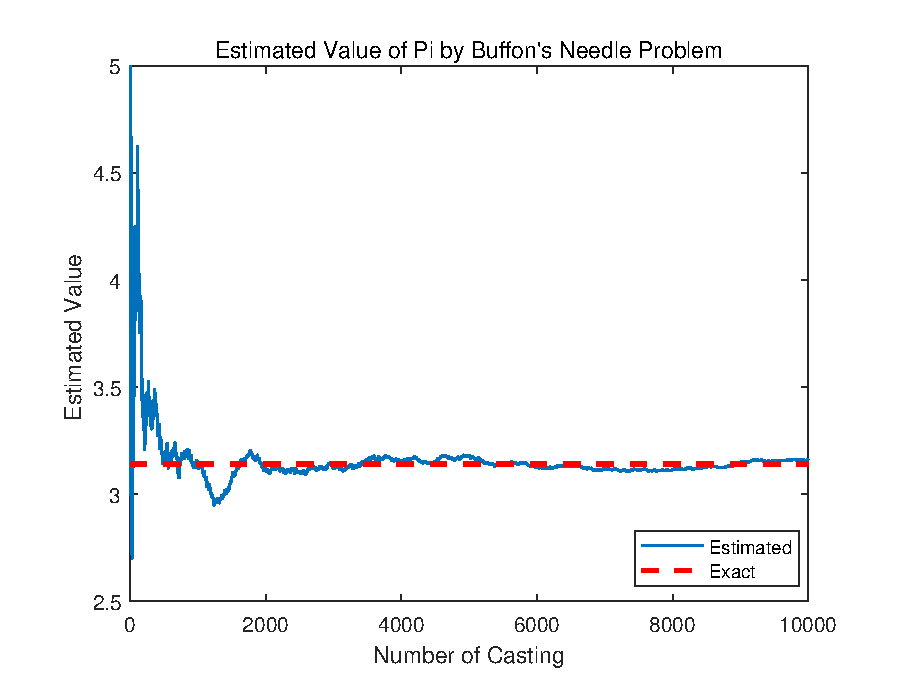
\includegraphics[width=1.1\textwidth]{Pi_N.eps}
        \caption{\fontsize{10pt}{15pt}\selectfont $\pi$估计值随投针次数N变化示意图}
    \end{minipage}
    \hspace{0cm}% 图片间距
    \hfill% 撑满整行
    \begin{minipage}{0.48\textwidth}
        \centering
        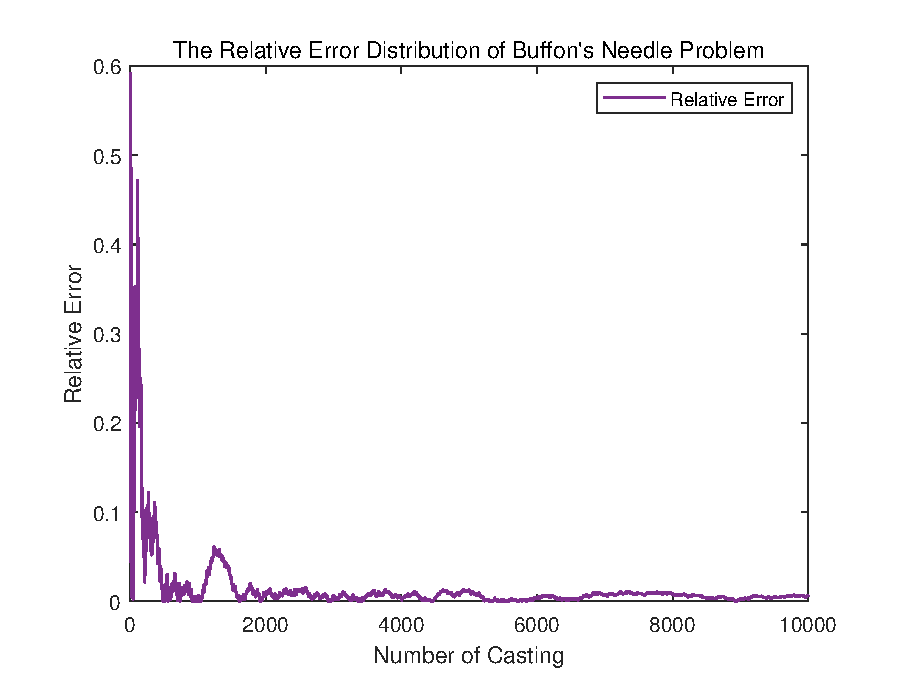
\includegraphics[width=1.1\textwidth]{Pi_N_Error.eps}
        \caption{\fontsize{10pt}{15pt}\selectfont $\pi$估计值随N变化相对误差分布图}
    \end{minipage}\label{fig:figure2}
\end{figure}

\subsubsection{问题$\left(c\right)$解答}
通过反复试验后我们可以发现MC方法计算$\pi$值虽然思想简洁直观,但是在占用相同内存的情况下,估计值的精度远不如级数展开法,可能有以下原因:

1.首先是随机数的选取,本文所采取的随机数为random库中的随机数,其分布可能在较少随机数数量下并不能体现出均匀性,这也就导致最终计算得出的$\pi$值精度大打折扣,下图给出了random库自带函数在1000个样本点下的分布情况,我们可以发现其并不满足均匀情况。

2.统计方法本身的特点造成了这一现象。由于Monte Carlo方法的原理是通过大样本下,事件频率趋近事件概率的现象来估计未知参数,由于每次实验的结果不能确定,具有一定的随机性,所以会出现单次实验结果偏差较大的情况。所以应该进行多次实验,将每次实验结果求和取平均值来估计未知参数更为合理。

3.实验的精度很大程度上取决于样本量。如果样本量不够大,那么估计值的误差可能会很大。随着样本量的增加,估计值的精度会逐渐提高,但增加样本量也意味着需要更多的计算资源和时间。

4.实验的设计也会影响精度。例如,平行线之间的距离、针的长度和投掷的方式都会影响相交次数的计算。

\begin{figure}[htbp]
    \centering
    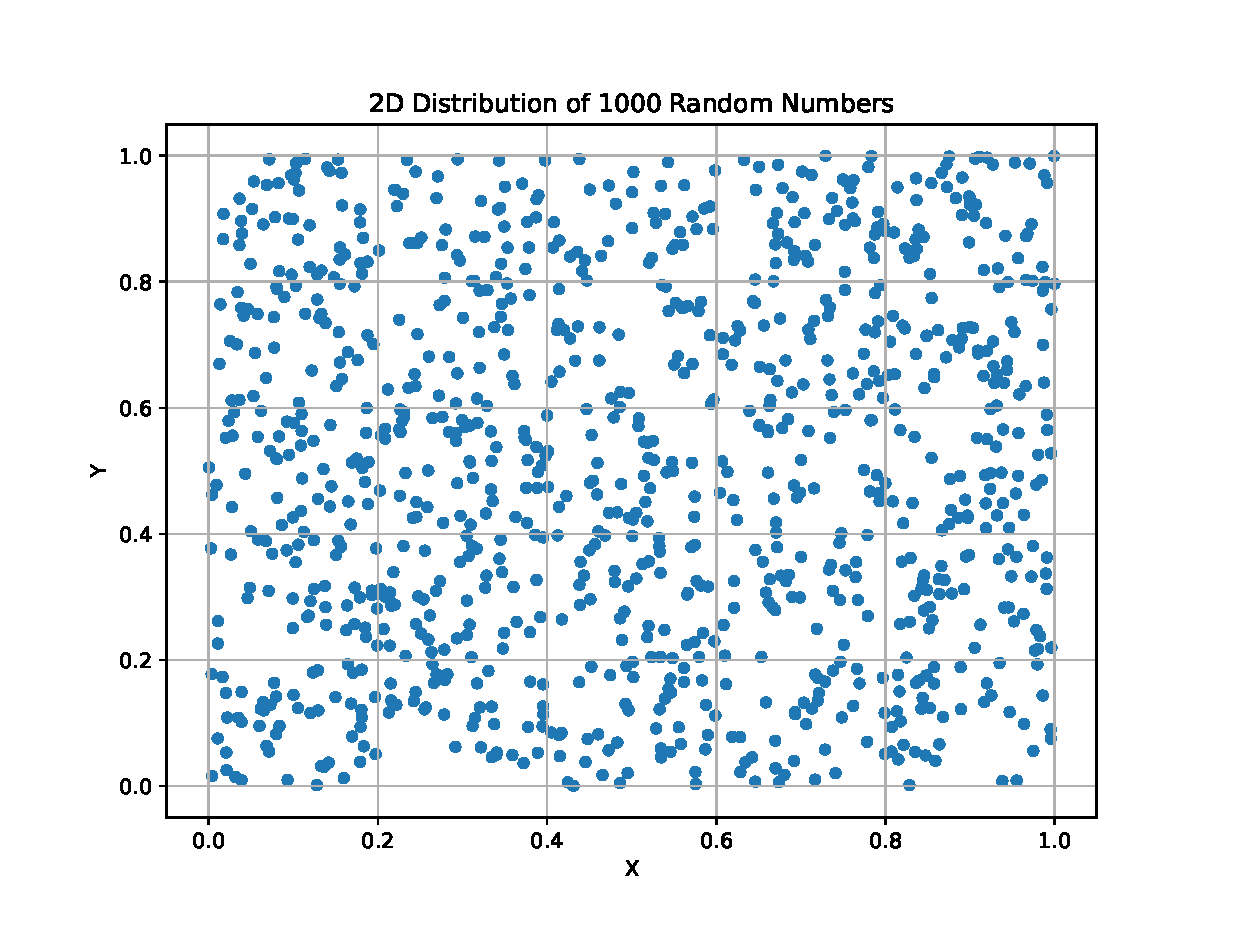
\includegraphics[height=8cm]{Random样本分布图.eps}\label{样本点分布图}
    \caption{1000个Random样本分布图}
\end{figure}

\subsubsection{问题$\left(d\right)$解答}

引入长针后,长度增加的针头的概率函数为:
\[P(x)=\left\{
    \begin{aligned}
         & \frac{2}{\pi}x                                      &  & x\leq 1 & \\
         & \frac{2}{\pi}\left(x-\sqrt{x^2-1}+arc \sec x\right) &  & x>1     &
    \end{aligned}
    \right.
\]

其中$x=\frac{b}{a}$是地板长度$a$和针长$b$的比值,对于地板长度$a$小于针长$b$的情况,我们同样可以得到$\pi$的估计公式:
\[\pi(x)=\frac{2}{P}\left(x-\sqrt{x^2-1}+arc\sec x \right)=N\frac{2}{k}\left(x-\sqrt{x^2-1}+arc\sec x\right)\]

经过编程后我们可以得到$\pi$的估计值随着长度比$x$的变化关系及其相对误差分布的图像:

\begin{figure}[H]% 插入两张图片并且并排
    \centering
    \begin{minipage}{0.48\textwidth}
        \centering
        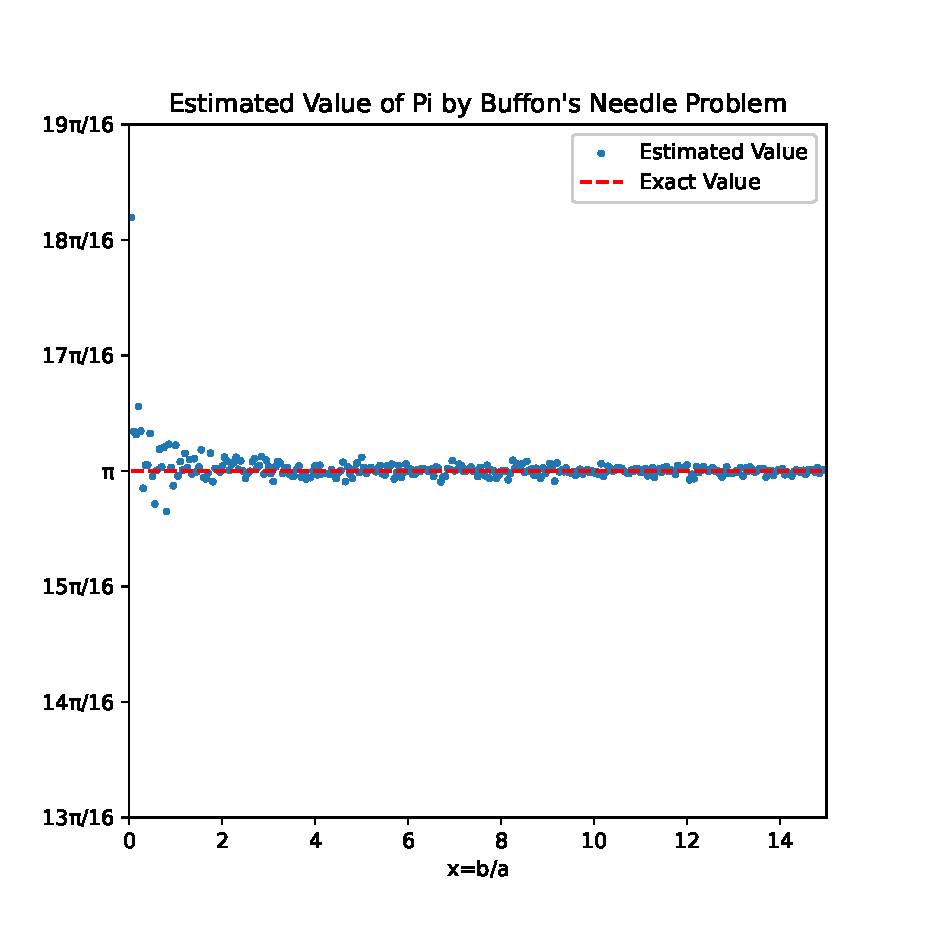
\includegraphics[width=1.1\textwidth]{Pi长短针估计值.eps}
        \caption{\fontsize{10pt}{15pt}\selectfont $\pi$估计值随$x$变化示意图}
    \end{minipage}
    \hspace{0cm}% 图片间距
    \hfill% 撑满整行
    \begin{minipage}{0.48\textwidth}
        \centering
        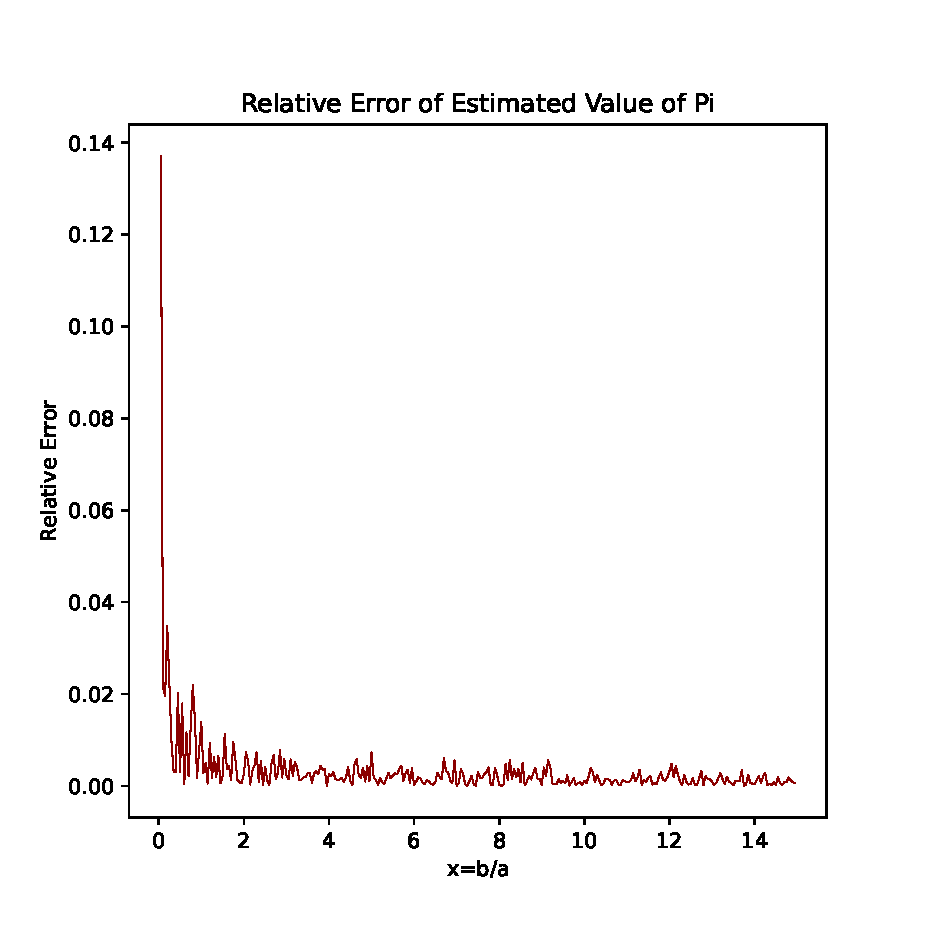
\includegraphics[width=1.1\textwidth]{Pi长短针估计值相对误差.eps}
        \caption{\fontsize{10pt}{15pt}\selectfont $\pi$估计值随$x$变化相对误差分布图}
    \end{minipage}\label{fig:figure2}
\end{figure}

\section{Problem 2}
\subsection{题目回顾}
使用传统的\textbf{Acceptance-Rejection Method}来计算$\pi$值。

$\left(a\right)$ 使用不同的N值来查看可以获得的精度大小。

$\left(b\right)$ 讨论一下为什么电脑只能达到这个精度?

\subsection{问题解答}

使用Acceptance-Rejection Method模拟实验来计算$\pi$的近似值,我选取了一些情况并对它们进行了可视化。

\begin{figure}[H]% 插入两张图片并且并排
    \centering
    \begin{minipage}{0.48\textwidth}
        \centering
        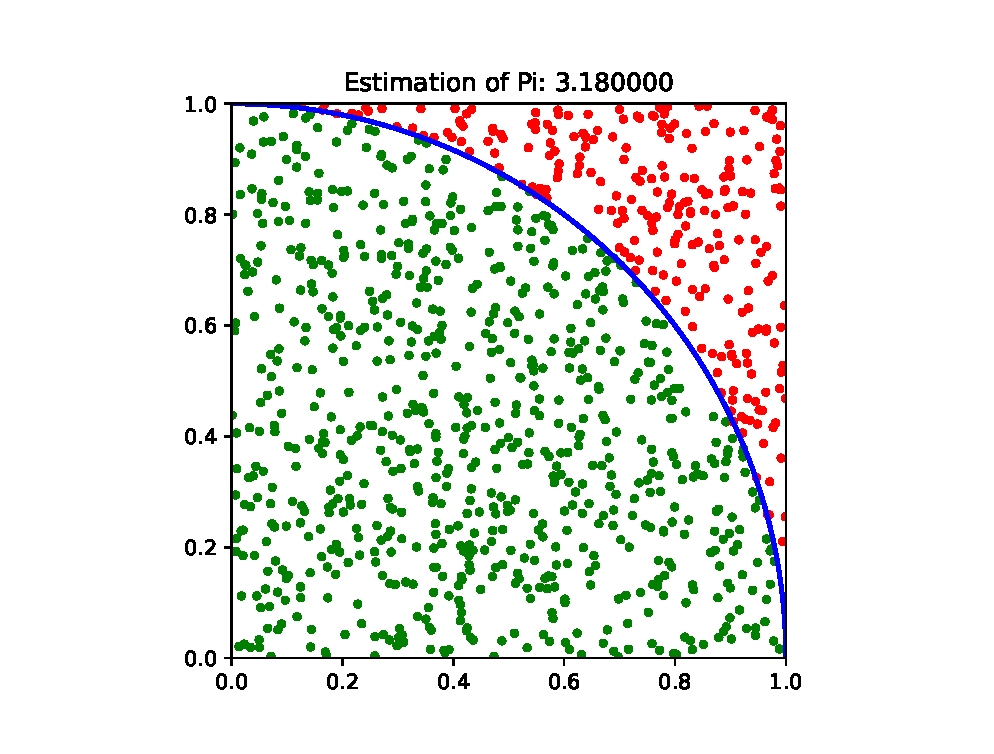
\includegraphics[width=1.1\textwidth]{pi_estimate_1000.eps}
        \caption{\fontsize{10pt}{15pt}\selectfont $\pi$的1000样本点示意图}
    \end{minipage}
    \hspace{0cm}% 图片间距
    \hfill% 撑满整行
    \begin{minipage}{0.48\textwidth}
        \centering
        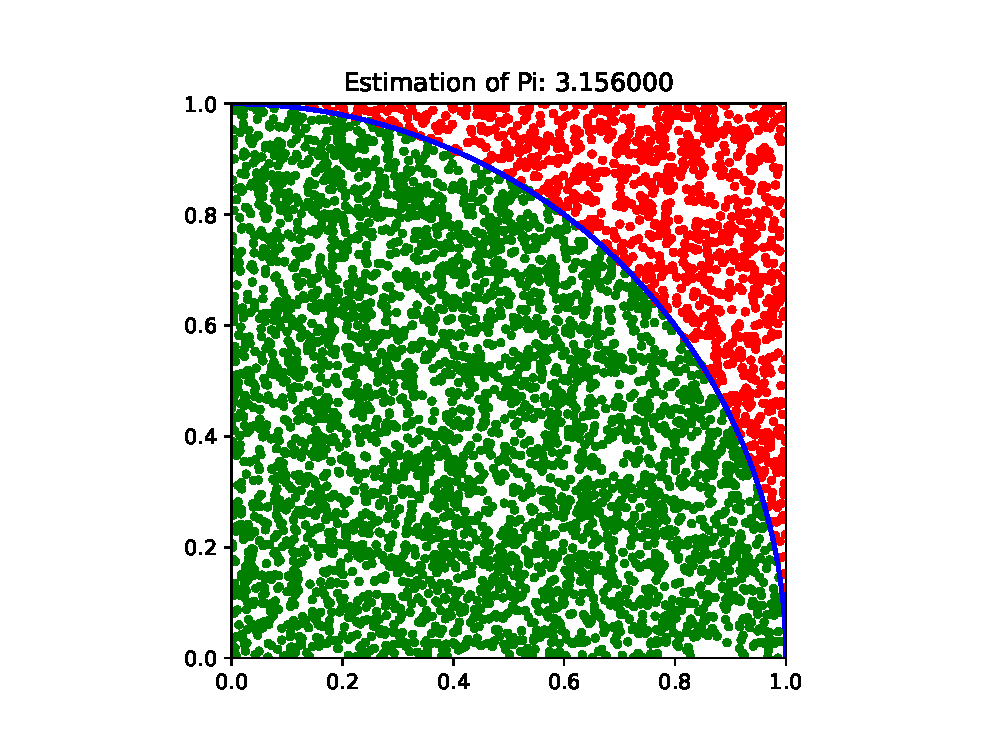
\includegraphics[width=1.1\textwidth]{pi_estimate_5000.eps}
        \caption{\fontsize{10pt}{15pt}\selectfont $\pi$的5000样本点示意图}
    \end{minipage}\label{fig:figure2}
\end{figure}

\begin{figure}[H]% 插入两张图片并且并排
    \centering
    \begin{minipage}{0.48\textwidth}
        \centering
        \includegraphics[width=1.1\textwidth]{pi_estimate_10000.png}
        \caption{\fontsize{10pt}{15pt}\selectfont $\pi$的10000样本点示意图}
    \end{minipage}
    \hspace{0cm}% 图片间距
    \hfill% 撑满整行
    \begin{minipage}{0.48\textwidth}
        \centering
        \includegraphics[width=1.1\textwidth]{pi_estimate_100000.png}
        \caption{\fontsize{10pt}{15pt}\selectfont $\pi$的100000样本点示意图}
    \end{minipage}\label{fig:figure2}
\end{figure}

具体试验结果列在下表中,可以观察到随着打靶次数N的增加,所得到的$\pi$的精度有统计规律上的增加趋势,但由于随机性,单次实验中,有可能出现N较小时的精度比N较大时的精度要高的情况,但是整体上呈现统计规律上的增加趋势。

%经典三线表
\begin{table}[H]
    \caption{\textbf{$\pi$估计值与相对误差}}%标题
    \centering%把表居中
    \begin{tabular}{ccc}%三个c代表该表一共三列,内容全部居中
        \toprule%第一道横线
        N        & Estimated value of $\pi$ & Relative Error \\
        \midrule%第二道横线 
        1000     & 3.176000                 & 0.010952       \\
        5000     & 3.156800                 & 0.004841       \\
        10000    & 3.162000                 & 0.006496       \\
        50000    & 3.152000                 & 0.003313       \\
        100000   & 3.143136                 & 0.000491       \\
        500000   & 3.141599                 & 0.000002       \\
        1000000  & 3.140476                 & 0.000355       \\
        5000000  & 3.141884                 & 0.000093       \\
        10000000 & 3.141018                 & 0.000183       \\
        \bottomrule      %第三道横线
    \end{tabular}
\end{table}

通过反复试验后我们可以发现MC方法计算$\pi$值虽然思想简洁直观,但是在占用相同内存的情况下,估计值的精度远不如级数展开法,可能有以下原因:

1.首先是随机数的选取,本文所采取的随机数为random库中的随机数,其分布可能在较少随机数数量下并不能体现出均匀性,这也就导致最终计算得出的$\pi$值精度大打折扣,下图给出了random库自带函数在1000个样本点下的分布情况,我们可以发现其并不满足均匀情况。

2.统计方法本身的特点造成了这一现象。由于Monte Carlo方法的原理是通过大样本下,事件频率趋近事件概率的现象来估计未知参数,由于每次实验的结果不能确定,具有一定的随机性,所以会出现单次实验结果偏差较大的情况。所以应该进行多次实验,将每次实验结果求和取平均值来估计未知参数更为合理。

3.实验的精度很大程度上取决于样本量。如果样本量不够大,那么估计值的误差可能会很大。随着样本量的增加,估计值的精度会逐渐提高,但增加样本量也意味着需要更多的计算资源和时间。

4.实验的设计也会影响精度。例如,平行线之间的距离、针的长度和投掷的方式都会影响相交次数的计算。

\section{Problem 3}
\subsection{题目回顾}
问题3:在黑暗时代,哈佛、达特茅斯和耶鲁只招收男生。假设当时,
1.哈佛男人80\%的儿子上了哈佛,其余的上了耶鲁,

2.耶鲁男性40\%的儿子上过耶鲁,其余的平均分配在哈佛和达特茅斯;

3.达特茅斯的人们\textbf{(此处题目疑似有错位,我们是按照自己的理解进行后续做答)}70\%去了达特茅斯,20\%去了哈佛,10\%去了耶鲁。

$\left(a\right)$  找出一个哈佛人的孙子上哈佛的概率。

$\left(b\right)$ 通过假设哈佛人的儿子总是上哈佛来修改上面的内容。再次找出一个哈佛人的孙子上哈佛的概率。

\subsection{问题解答}
\subsubsection{问题$\left(a\right)$解答}
取四维列向量,其各分量分别为 Harvard Yale Dartmouth woman 的概率

    对 (a) Markov 矩阵如下
    \begin{equation*}
        T = \left( \begin{matrix*}
                       0.40 & 0.15 & 0.15 & 0.35 \\
                       0.00 & 0.20 & 0.20 & 0.10 \\
                       0.10 & 0.15 & 0.15 & 0.05 \\
                       0.50 & 0.50 & 0.50 & 0.50 \\
        \end{matrix*} \right)
    \end{equation*}

    对 (b) Markov 矩阵如下
    \begin{equation*}
        T = \left( \begin{matrix*}
                       0.50 & 0.15 & 0.15 & 0.35 \\
                       0.00 & 0.20 & 0.20 & 0.10 \\
                       0.00 & 0.15 & 0.15 & 0.05 \\
                       0.50 & 0.50 & 0.50 & 0.50 \\
        \end{matrix*} \right)
    \end{equation*}

    所求均为计算
    \begin{equation*}
        T^2 \left( \begin{matrix*}
                       1 \\ 0 \\ 0 \\ 0 \\
        \end{matrix*} \right)
    \end{equation*}
    的第一个元素。

    用 \texttt{Java} 代码实现,见附件 \texttt{MatrixCal1.java},运行结果如下
    \begin{figure}[h]
        \centering
        \includegraphics[height=0.05 \textheight]{prob_3}
        \caption{MatrixCal1 运行结果}\label{fig:figure3}
    \end{figure}

\section{Problem 4}
\subsection{题目回顾}
一只老鼠穿过下面的迷宫。在每走一步的时候,它都会随机选择一扇门离开房间

$\left(a\right)$ 给出这个Markoy链的转移矩阵P

$\left(b\right)$ 证明它是不可约的,但不是非周期的

$\left(c\right)$ 找到平稳分布

$\left(d\right)$ 现在假设一块成熟的切达干酪被放在5号房间的一个致命陷阱上。鼠标在1号房间启动。从1号房间开始,在第一次到达5号房间之前找到预期的步数

$\left(e\right)$ 找到返回1号房间的预期时间
\subsection{问题解答}
\subsubsection{问题$\left(a\right)$解答}
Markov链的转移矩阵为:

\begin{gather*}
    \begin{bmatrix}
        0 & 0 & \frac{1}{4} & 0           & 0           & 0           \\
        0 & 0 & \frac{1}{4} & 0           & 0           & 0           \\
        1 & 1 & 0           & \frac{1}{2} & \frac{1}{2} & 0           \\
        0 & 0 & \frac{1}{4} & 0           & 0           & \frac{1}{2} \\
        0 & 0 & \frac{1}{4} & 0           & 0           & \frac{1}{2} \\
        0 & 0 & 0           & \frac{1}{2} & \frac{1}{2} & 0
    \end{bmatrix}
\end{gather*}

\subsubsection{问题$\left(b\right)$解答}
考虑在该 Markov 链中的多个时间,用 \texttt{Java} 代码实现,见附件 \texttt{MatrixCal2.java},运行结果如下

    \begin{figure}[H]% 插入两张图片并且并排
        \centering
        \begin{minipage}{0.48\textwidth}
            \centering
            \includegraphics[width=1.1\textwidth]{prob_4_2_1.png}
            \caption{\fontsize{10pt}{15pt}\selectfont 从 room1 出发}
        \end{minipage}
        \hspace{0cm}% 图片间距
        \hfill% 撑满整行
        \begin{minipage}{0.48\textwidth}
            \centering
            \includegraphics[width=1.1\textwidth]{prob_4_2_2.png}
            \caption{\fontsize{10pt}{15pt}\selectfont 初始各 room 概率相等}
        \end{minipage}\label{fig:figure2}
    \end{figure}

    可见,当时间足够长后,呈现一定的周期分布,不同的初始导向不同的循环。

\subsubsection{问题$\left(c\right)$解答}
利用 \texttt{matlab} 计算特征向量,实现如下

结果即 \(J\) 中 \(1\) 的值在 \(V\) 中对应的列(归一化后)
\begin{equation*}
    \eta_0 = \left( \begin{matrix*}
                        \frac{1}{10} \\
                        \frac{1}{10} \\
                        \frac{2}{5}  \\
                        \frac{1}{5}  \\
                        \frac{1}{5}  \\
                        \frac{1}{5}  \\
    \end{matrix*} \right)
\end{equation*}

\subsubsection{问题$\left(d\right)$解答}
该问题即到达 room 5 后,到其他 room 的概率全为 0,对转移矩阵作以下调整
\begin{equation*}
    P = \left( \begin{matrix*}
                   0 & 0 & \frac{1}{4} & 0           & 0 & 0 \\
                   0 & 0 & \frac{1}{4} & 0           & 0 & 0 \\
                   1 & 1 & 0           & \frac{1}{2} & 0 & 0 \\
                   0 & 0 & \frac{1}{4} & 0           & 0 & \frac{1}{2} \\
                   0 & 0 & \frac{1}{4} & 0           & 0 & \frac{1}{2} \\
                   0 & 0 & 0           & \frac{1}{2} & 0 & 0 \\
    \end{matrix*} \right)
\end{equation*}
再利用 \texttt{Java} 代码计算均值即可,见附件 \texttt{MatrixCal2.java}(设置 \texttt{index = 4})。

观察得,在一定的时间后,均值稳定在 6.000000000000003,此时 room 5 的概率已经趋近于 0。

\subsubsection{问题$\left(e\right)$解答}
该问题即到达 room 1 后,到其他 room 的概率全为 0,对转移矩阵作以下调整
    \begin{equation*}
        P = \left( \begin{matrix*}
                       0 & 0 & \frac{1}{4} & 0           & 0           & 0 \\
                       0 & 0 & \frac{1}{4} & 0           & 0           & 0 \\
                       0 & 1 & 0           & \frac{1}{2} & \frac{1}{2} & 0 \\
                       0 & 0 & \frac{1}{4} & 0           & 0           & \frac{1}{2} \\
                       0 & 0 & \frac{1}{4} & 0           & 0           & \frac{1}{2} \\
                       0 & 0 & 0           & \frac{1}{2} & \frac{1}{2} & 0 \\
        \end{matrix*} \right)
    \end{equation*}
    再利用 \texttt{Java} 代码计算均值即可,见附件 \texttt{MatrixCal2.java}(设置 \texttt{index = 0})。

    观察得,在一定的时间后,均值稳定在 10.999999999999996,此时 room 1 的概率已经趋近于 0。
    


\section{Problem 5}
\subsection{题目回顾}
考虑一个矩形网格,垂直线间隔a个单位,水平线间隔b个单位。长度$l<min(a,b)$的针随机落在网格上,设A表示针穿过垂直线的事件,设B表示针穿过水平线的事件。

$\left(a\right)$  $P(A)=2l/(\pi a)$

$\left(b\right)$  $P(B)=2l/(\pi b)$

$\left(c\right)$  $P(A\cap  B)=l^2/(\pi ab)$

利用传统的MC方法,使用上述三种公式来模拟蒲丰投针问题,计算$\pi$。哪一种能得到最好的结果,绘制(c)的结果。

\subsection{问题解答}

当夹角为$\theta$时,针的纵向长度为$l \sin \theta$,横向长度$l\cos\theta$

与纵向线相交的概率 \(\frac{l \cos{\theta}}{a}\),与横向线相交的概率 \(\frac{l \sin{\theta}}{b}\),两条都相交的概率为 \(\frac{l^2 \sin{\theta} \cos{\theta}}{ab}\)。

对角度的均值
\begin{equation*}
    \begin{align*}
        P(A) & = \frac{1}{\pi / 2} \int_{0}^{\pi / 2} \frac{l \cos{\theta}}{a} d \theta \\
        & = \frac{2l}{\pi a} \\
        P(B) & = \frac{1}{\pi / 2} \int_{0}^{\pi / 2} \frac{l \sin{\theta}}{b} d \theta \\
        & = \frac{2l}{\pi b} \\
        P(C) & = \frac{1}{\pi / 2} \int_{0}^{\pi / 2} \frac{l^2 \sin{\theta} \cos{\theta}}{ab} d \theta \\
        & = \frac{2l^2}{\pi ab} \\
    \end{align*}
\end{equation*}

利用 \texttt{Java} 代码实现上述问题的计算,见附件 \texttt{Buffon2D.java},运行结果如下

\begin{figure}[H]% 插入两张图片并且并排
    \centering
    \begin{minipage}{0.48\textwidth}
        \centering
        \includegraphics[width=1.1\textwidth]{prob_5_2.png}
        \caption{\fontsize{10pt}{15pt}\selectfont Buffon2D 运行结果}
    \end{minipage}
    \hspace{0cm}% 图片间距
    \hfill% 撑满整行
    \begin{minipage}{0.48\textwidth}
        \centering
        \includegraphics[width=1.1\textwidth]{prob_5_3.png}
        \caption{\fontsize{10pt}{15pt}\selectfont Buffon2D 运行结果}
    \end{minipage}\label{fig:figure2}
\end{figure}

对比回归斜率,2维并没有明显优势,不过略微有提高收敛速度。

\end{document}% 结束文档编辑,后面写啥都编译不出来